
\subsection{Laser \todo{1x}}\label{k4:laser}
    \subsubsection{Wie funktionieren HL-Laser?}
    Licht kann von Halbleitern absorbiert und emittiert werden.
    Es gilt die Energieerhaltung: $\hbar \omega = \Delta E$, mit der Kreisfrequenz des absorbierten bzw. emittierten Lichts $\omega$,
    und der Energiedifferenz zwischen Anfangs- und Endzustand des Elektrons $\Delta E$.\\
    Es gibt
    \begin{enumerate}
        \item \emph{Interband\"uberg\"ange}, also \"Uberg\"ange zwischen zwei verschiedenen B\"andern
        \item \emph{Intraband\"uberg\"ange} innerhalb eines Bandes zwischen zwei verschiedenen Energieniveaus
    \end{enumerate}
    Die Wechselwirkung zwischen Elektronen und Photonen kann auf drei Arten geschehen:
    \begin{enumerate}
        \item \emph{Absorption}: Ein Photon mit der richtigen Energie kann in einem quanten-mechanischen System (mit einer gewissen Wahrscheinlichkeit) ein Elektron von einem niederenergetischen Zustand in einen höherenergetischen Zustand heben. Das Photon wird
        dabei vernichtet.
        \item \emph{Spontane Emission}: Ein Elektron in einem angeregten Zustand eines quanten-mechanischen Systems kann spontan ein Photon emittieren. Das Elektron fällt dabei vom höherenergetischen in den niederenergetischen Zustand. So funktionieren LEDs.
        \item \emph{Stimulierte Emission}: Trifft ein Photon auf ein angeregtes System, so kann (mit einer gewissen Wahrscheinlichkeit) ein zweites (identes) Photon erzeugt werden. Das Elektron fällt dabei vom höherenergetischen in den niederenergetischen Zustand.
        So funktionieren LASER (\textbf{L}ight \textbf{a}mplification by \textbf{s}timulated \textbf{e}mission of \textbf{r}adiaton).
    \end{enumerate}
    Beispielhafter Aufbau eines HL-Lasers in \Cref{fig:hlLaser}.
    \begin{figure}[H]
        \centering
        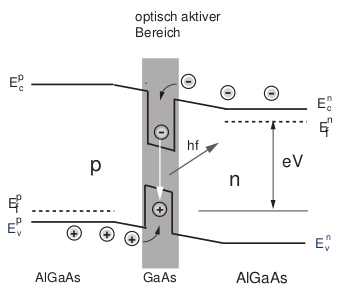
\includegraphics[width=0.6\textwidth]{fig/hlLaser}
        \caption{Aufbau eines HL-Lasers}
        \label{fig:hlLaser}
    \end{figure}
    Die Laserstrahlung liegt energetisch unter der Bandlücke des umgebenden Materials. Die Strahlung kann also problemlos aus dem Halbleiter heraus und wird nicht wieder absorbiert.
    \subsubsection{E(k) Diagramm}
        \begin{figure}[H]
            \centering
            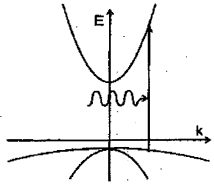
\includegraphics[width=0.3\textwidth]{fig/ekLaser}
            \caption{E(k)-Diagramm f\"ur Laser}
            \label{fig:ekLaser}
        \end{figure}
    \subsubsection{stimulierte Emission}
    Im thermodynamischen Gleichgewicht tritt stets Absorption auf ($Uv(E_1)-f_c(E_2) > 0$), nicht aber wenn der Halbleiter angeregt wird ($Uv(E_1)-f_c(E_2) < 0$), man spricht von Inversion.
    \subsubsection{Verst\"arkerbedingung}
    $E_{F_C}$ Fermi-Niveau Leitungsband\\
    $E_{F_V}$ Fermi-Niveau Valenzband\\
    Bedingung: $E_{F_C} - E_{F_V} > E_G$. ???\\
    Bei $T=0K$ genügt eine beliebig kleine Ladungsträgerinjektion, um die Quasi-Fermi-Niveaus $E_{F_c}$ und $E_{F_v}$ in die Bänder hinein zu verschieben (\Cref{fig:invLaser}) und die Verstärkerbedingung zu erfüllen. Bei Raumtemperatur ist allerdings eine relativ hohe Mindestladungsträgerdichte erforderlich, um Inversion zu erreichen ($ > 10^{18}/cm^3$).
        \begin{figure}[H]
            \centering
            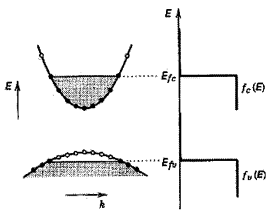
\includegraphics[width=0.3\textwidth]{fig/inversionLaser}
            \caption{Inversion bei $T=0K$}
            \label{fig:invLaser}
        \end{figure}

\subsection{Vergleiche direkte und indirekte Halbleiter \todo{1x}}\label{k4:inUndIndirekt}
    Bei direkten Halbleitern liegt das Maximum des Valenzbandes energetisch genau unter dem Minimum des Leitungsbandes, dies ist z.B. bei
    Galliumarsenid der Fall. Bei indirekten Halbleitern liegen diese ausgezeichneten Punkte bei unterschiedlichen k-Werten (Silizium, Germanium).
    \subsubsection{Wo ist k=0, was bedeutet das?}
    Beim direkten Halbleiter ist $k=0$ dort, wo das minimum des Leitungsbandes und das maximum des Valenzbandes liegen. Sonst???
    \subsubsection{w(k) für freies Teilchen}
    ???
    \subsubsection{Bewegt sich ein e- im Ev bei T=0?}
    ?\\
    Nein, bei $0K$ ist das Valenzband voll besetzt. Elektronen k\"onnen sich nirgends hin bewegen.
    \subsubsection{Wo ist die Masse am größten (Ev, Ec)?}
    ???
    \subsubsection{Gleichung für m*}
    Aufgrund der Auswirkung der Bandstruktur auf die Elektronen im Kristall scheinen diese dort eine andere Masse zu haben, sie wird
    effektive Masse $m^{*}$ genannt.
    \begin{equation}
        \frac{1}{m^{*}} = \frac{1}{\hbar^2}*\frac{d^2E}{dk^2}
    \end{equation}
    \begin{figure}
        \centering
        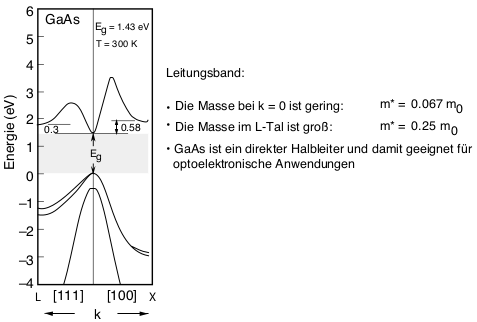
\includegraphics[width=0.8\textwidth]{fig/bandstrukturGaAs}
        \caption{Bandstruktur GaAs}
        \label{fig:bandGaAs}
    \end{figure}
    Betrachtet man die Bandstruktur von z.B. GaAs (\Cref{fig:bandGaAs}), erkennt man dass bei den Wendepunkten die Masse ins unendliche
    gehen w\"urde. Dies passiert aber nicht, in diesen Gebieten braucht es ein anderes Modell, die kp-Theorie.
    Am oberen Rand wird die effektive Masse negativ. Man spricht von einem Loch, die Ladung wird positiv.

\subsection{Zustandsdichte und Besetzungswahrscheinlichkeit \todo{2x}}\label{k4:zustandsDichte}
    Quantensysteme haben diskrete Zust\"ande.
    Die Zustandsdichte $g(E) = \frac{N}{L^3}$ gibt an wie viele Zust\"ande pro eV es zu einem gewissen Energieniveau gibt (Mit $N$ anzahl diskreter Zust\"ande, $L^3$ Volumen des HL).
    Die Besetzungswahrscheinlichkeit, auch Fermi-Verteilung, $P(E)$ gibt die Wahrscheinlichkeit an dass ein Zustand eingenommen wurde.
    Daraus l\"asst sich berechnen, wie viele Leitungstr\"ager vorhanden sind: $n = \int{g(E)*P(E) dE}$
    
    \subsubsection{Banddiagramme}
    ???
    \subsubsection{Temperaturabh\"angigkeit}
    Die Fermi-Verteilung ist Temperaturabh\"angig. Desto nidriger die Temperatur, desto steiler f\"allt die Verteilung ab.
    \begin{figure}[H]
        \centering
        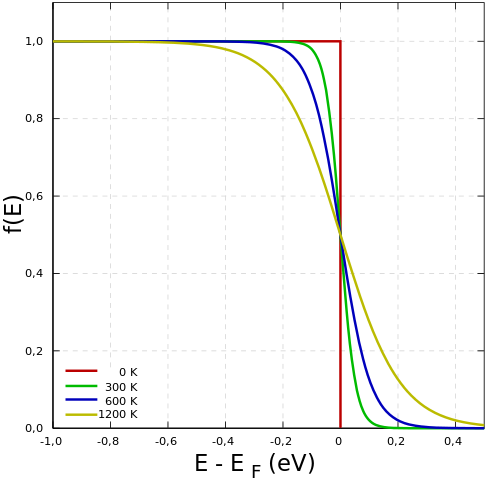
\includegraphics[width=0.5\textwidth]{fig/fermi}
        \caption{Fermi-Verteilung}
        \label{fig:fermi}
    \end{figure}